\chapter{Arhitektura i dizajn sustava}

\begin{figure}[H]
	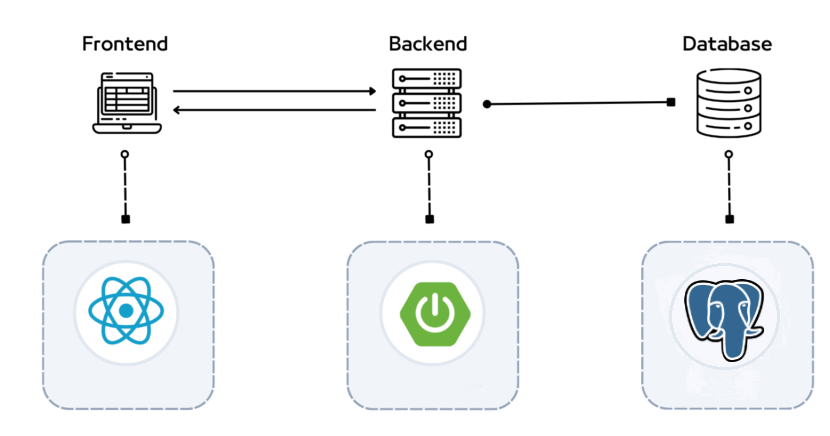
\includegraphics[scale=1]{slike/prikaz_arhitekture.png}
	\centering
	\caption{Prikaz arhitekture sustava}
\end{figure}

Arhitektura sustava može se podijeliti na tri glavna podsustava, a to su \textbf{Web poslužitelj, Web aplikacija i baza podataka}.
\begin{itemize}
	\item 	\textit{\textbf{Web poslužitelj}} prima zahtjeve od klijenata putem interneta, obrađuje ih i pruža resurse poput web stranice, slike, videa i datoteke kao odgovor. Za distribuciju resursa najčešče se koriste protokoli kao što su HTTP (Hypertext Transfer Protocol) ili HTTPS (HTTP Secure).
	\item 	\textit{\textbf{Web aplikacija}} je program koji se izvršava na web pregledniku (Google Chrome, Mozilla Firefox, Safari itd.) i pruža korisnicima mogućnost izvršavanja željenih zahtjeva, odnosno interakciju s određenim uslugama i funkcionalnostima web aplikacije. Prilikom obrade zahtjeva pristupa se bazi podataka i korisniku se odgovor vraća kao HTML dokument.
	\item 	\textit{\textbf{Baza podataka}} je organizirani skup podataka namijenjen za efikasno upravljanje, ažuriranje, pretraživanje i dohvat podataka. Uloge baze podataka u web aplikaciji su pohrana podataka, očuvanje integriteta podataka i osiguravanje dosljednosti, upravljanje transakcijama itd.
\end{itemize}

Za izradu naše web aplikacije odabrali smo \textit{\textbf{Spring Boot}} (open-source Java framework) i \textit{\textbf{React}} (open-source JavaScript library). Odabrana razvojna okruženja su InteliJ IDEA i Eclipse IDE za Spring Boot, odnosno Visual Studio Code i WebStorm za React. Za izradu baze podatka koristimo PostgreSQL.
Arhitektura, koja je podržana Spring Boot-om, temelji se na \textit{\textbf{MVC (Model-View-Controller)}} konceptu koji strogo odvaja model, akcije i prezentaciju, olakšava razvoj i održavanje aplikacije te čini aplikaciju prilagodljivom i jednostavnom za proširenje.
\begin{itemize}
	\item \textit{\textbf{Model}} - predstavlja poslovnu logiku, odnosno dinamičke strukture podataka, mijenja pogled na zahtjev kontrolera. Modeli u pravilu predstavljaju podatke(objekte) koje aplikacija obrađuje.
	\item \textit{\textbf{View}} - ono što klijent vidi, odnosno korisničko sučelje potrebno za interakciju s aplikacijom kao što su dijagrami, linkovi, slike, tablice itd.
	\item \textit{\textbf{Controller}} - presreće zahtjeve klijenata i prilagođava model, odnosno obavještava model o promjeni zahtjeva korisnika i u skladu sa zahtjevima daje prikladan View.
\end{itemize}




\section{Baza podataka}

\textbf{\textit{dio 1. revizije}}\\

\textit{Potrebno je opisati koju vrstu i implementaciju baze podataka ste odabrali, glavne komponente od kojih se sastoji i slično.}

\subsection{Opis tablica}


\textit{Svaku tablicu je potrebno opisati po zadanom predlošku. Lijevo se nalazi točno ime varijable u bazi podataka, u sredini se nalazi tip podataka, a desno se nalazi opis varijable. Svjetlozelenom bojom označite primarni ključ. Svjetlo plavom označite strani ključ}


\begin{longtblr}[
	label=none,
	entry=none
	]{
	width = \textwidth,
	colspec={|X[6,l]|X[6, l]|X[20, l]|},
	rowhead = 1,
	} %definicija širine tablice, širine stupaca, poravnanje i broja redaka naslova tablice
	\hline \SetCell[c=3]{c}{\textbf{korisnik - ime tablice}}                                                           \\ \hline[3pt]
	\SetCell{LightGreen}IDKorisnik & INT     & Lorem ipsum dolor sit amet, consectetur adipiscing elit, sed do eiusmod \\ \hline
	korisnickoIme                  & VARCHAR &                                                                         \\ \hline
	email                          & VARCHAR &                                                                         \\ \hline
	ime                            & VARCHAR &                                                                         \\ \hline
	\SetCell{LightBlue} primjer    & VARCHAR &                                                                         \\ \hline
\end{longtblr}


\pagebreak
\subsection{Dijagram baze podataka}
\textit{ U ovom potpoglavlju potrebno je umetnuti dijagram baze podataka. Primarni i strani ključevi moraju biti označeni, a tablice povezane. Bazu podataka je potrebno normalizirati. Podsjetite se kolegija "Baze podataka".}
\begin{figure}[H]
	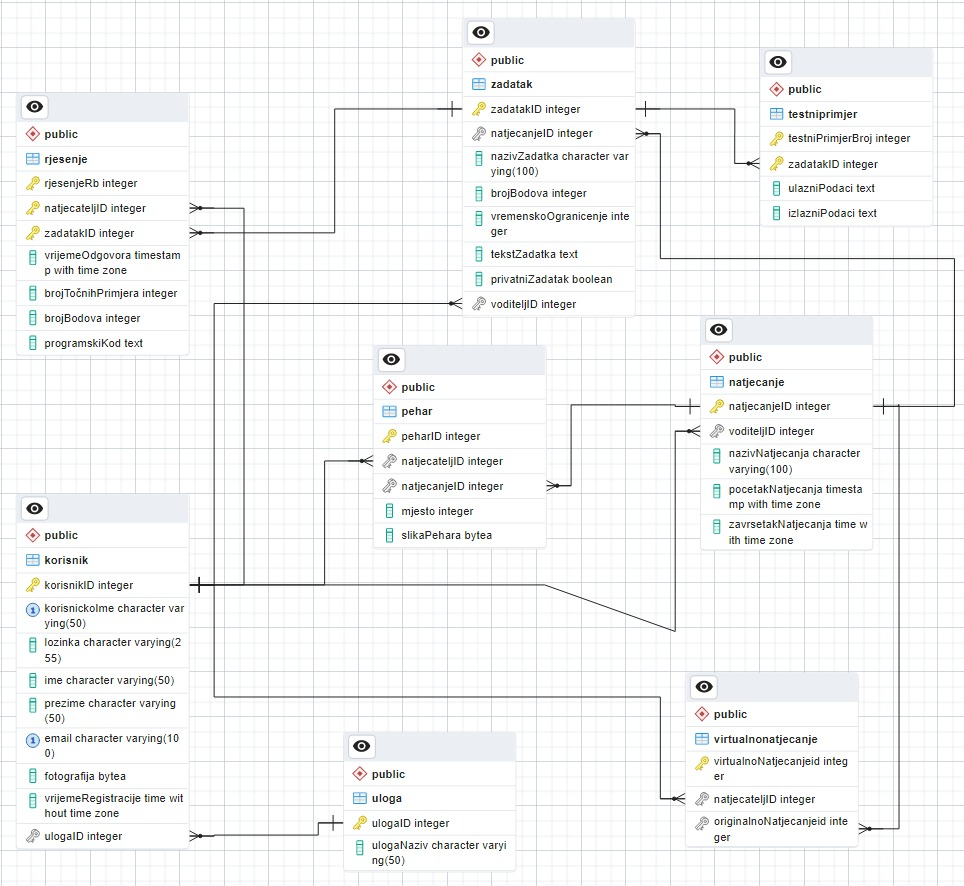
\includegraphics[scale=0.4]{dijagrami/dijagram_baze_podataka.jpeg} 
	\centering
	\caption{Dijagram baze podataka}
	\label{fig:bazaPodataka} 
\end{figure}

\eject


\section{Dijagram razreda}

\textit{Potrebno je priložiti dijagram razreda s pripadajućim opisom. Zbog preglednosti je moguće dijagram razlomiti na više njih, ali moraju biti grupirani prema sličnim razinama apstrakcije i srodnim funkcionalnostima.}\\

\textbf{\textit{dio 1. revizije}}\\

\textit{Prilikom prve predaje projekta, potrebno je priložiti potpuno razrađen dijagram razreda vezan uz \textbf{generičku funkcionalnost} sustava. Ostale funkcionalnosti trebaju biti idejno razrađene u dijagramu sa sljedećim komponentama: nazivi razreda, nazivi metoda i vrste pristupa metodama (npr. javni, zaštićeni), nazivi atributa razreda, veze i odnosi između razreda.}\\

\textbf{\textit{dio 2. revizije}}\\

\textit{Prilikom druge predaje projekta dijagram razreda i opisi moraju odgovarati stvarnom stanju implementacije}



\eject

\section{Dijagram stanja}


\textbf{\textit{dio 2. revizije}}\\

\textit{Potrebno je priložiti dijagram stanja i opisati ga. Dovoljan je jedan dijagram stanja koji prikazuje \textbf{značajan dio funkcionalnosti} sustava. Na primjer, stanja korisničkog sučelja i tijek korištenja neke ključne funkcionalnosti jesu značajan dio sustava, a registracija i prijava nisu. }


\eject

\section{Dijagram aktivnosti}

\textbf{\textit{dio 2. revizije}}\\

\textit{Potrebno je priložiti dijagram aktivnosti s pripadajućim opisom. Dijagram aktivnosti treba prikazivati značajan dio sustava.}

\eject
\section{Dijagram komponenti}

\textbf{\textit{dio 2. revizije}}\\

\textit{Potrebno je priložiti dijagram komponenti s pripadajućim opisom. Dijagram komponenti treba prikazivati strukturu cijele aplikacije.}